\chapter{Software System}
In the following chapter, we are going to discuss the development of the software system used to conduct the experiments described later in this thesis. First, we are going to describe the basic requirements for such a system and then go into the ''story'' behind the development, show where we have been stuck and how we solved this problems. Then we are going to describe the environment in which this software system can be used and what kind of external software and hardware was used to run the experiments on.

\section{Requirements}
We started the development of the system by defining which requirements it has to fulfill in order to be suitable for conducting the experiments of this thesis. The following properties were identified which the developed system should fulfill:

\begin{itemize}
	\item \textbf{Parameterizable}: All experiments should be allowed to run in parameterized manner, which means that all important hyperparameters, training data and places to store the different results should be parameterizable through a JSON\footnote{http://www.json.org/} configuration file.
	\item \textbf{Reproducable}: It should be possible to run experiments multiple times without having to put additional efforts into it.
	\item \textbf{Analyzable}: This means that all results from all experiments should be stored in a distinct place for analysis later. This includes the trained models, all metrics collected while training and also the configuration used.
	\item \textbf{Recoverable}: Due to the fact, that we knew that the environment in which the experiments were going to be conducted (see chapter \ref{} on the hardware) is kind of volatile with regard to stability, we decided that we must design the system in such a way, that the unexpected termination of a running experiment should be easily recoverable. This means, that it should be possible to load the most recent model from the previous training and go on from the point where the training was interrupted. This includes loading and saving of the model weights, skipping all of the training data the model was already trained on as well as loading all the metric already collected in the first run.
	\item \textbf{Evaluatable}: The trained models should be easily evaluatable, which means that we should have a way of doing inference without the hassle to load the stored configurations and models by hand. The most comfortable way of doing this is through a small frontend which provides the possiblity to ''speak'' to a trained model.
\end{itemize}

The properties listed above should be fulfilled by the newly developed system in order to enable us to safely conduct experiments without the fear of loosing out on any of the results.

\section{Development of the System}
\begin{itemize}
	\item Why we've switch from Keras to Tensorflow
	\item Beginning was really hard, as TF is much more low level than keras
	\item Had huge problems due to different seq2seq APIs with different levels of documentation, bug-freenes and future-support.
	\item Google Seq2Seq Tool -> Inference broken
	\item Settled with legacy API as we know this one is working
\end{itemize}
\section{Model Validation Checks}
\label{software_sytem:model_validation_checks}
As described in the section before, we were struggling with the development of the software system, especially with the construction of the TensorFlow graph itself. We have had a lot of setbacks and hence were not sure how to validate that our latest model is working without spending several days to weeks on training before noticing that the graph is still broken. For this reason, we have developed two so-called model validation checks, which should ensure that the model is not broken before starting the large, long-running experiments.

The first validation we introduced was a simple copy-page task: The model was trained to copy sequences of integers of different lengths. For this purpose, we have generated a dataset of $10'000$ sequences of random length and random content. We have used the integers from $0$ to $19$ as the vocabulary and the generated sequences were between $1$ and $40$ symbols long. We then used the implemented model and trained it to output the exact input sequence, for which we used the aforementioned random integer sequences. 

The second validation was a simple overfitting test: The model was fed with tweets as input sequences and the respective response as output sequences. For this purpose we have used a dataset of english tweets borrowed from the user ''Marsan-Ma'' on GitHub\footnote{https://github.com/Marsan-Ma/chat\_corpus/}. We conditioned the model to output the expected output sequence each time we have used a specific input sequence.

Through using these two validation checks, we were able to gain confidence that the implemented model works as expected without using as much time as a full training on any of the conversational datasets would have required.

\section{Scripts}
\begin{itemize}
	\item Explain what we've used scripts for
\end{itemize}
\section{Web-UI}
We have also developed an elementary GUI for doing inference through a web frontend. This allowed us to interact with the models after they have been trained in a quick and easy way. We have used the python web framework \texttt{flask}\footnote{http://flask.pocoo.org/} for implementing the backend system and a combination of \texttt{jQuery}\footnote{https://jquery.com/} JavaScript library and the \texttt{boostrap}\footnote{http://getbootstrap.com/} frontend framework.

\begin{figure}[h]
	\label{fundamentals:lstm:internal_structure}
	\centering
	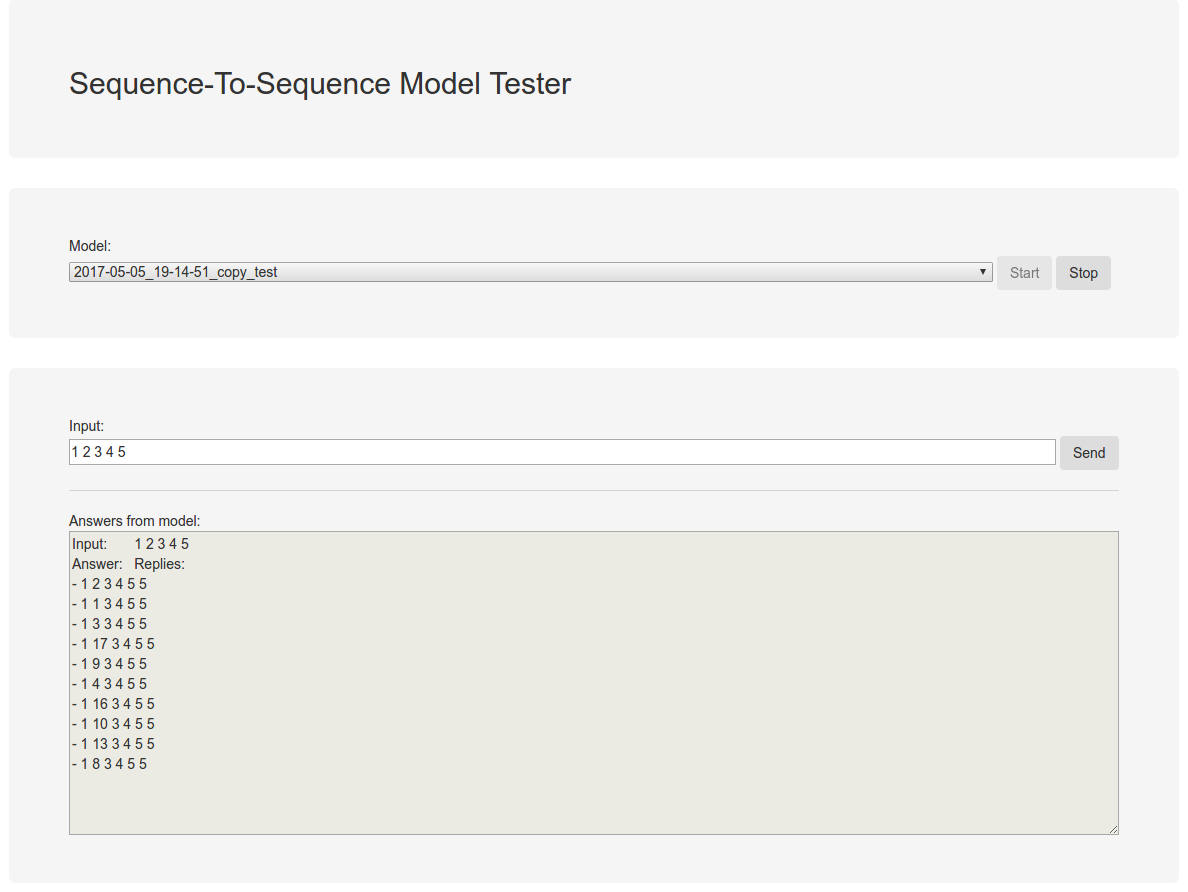
\includegraphics[width=10cm]{img/web_frontend_inference}
	\caption{Frontend showing the output when sending the sequence ''1 2 3 4 5'' to a model trained on the copy task (see chapter \ref{software_sytem:model_validation_checks}).}
\end{figure}

\section{Operating System \& Software Packages}
\begin{itemize}
	\item Declare all dependencies and how the system has to be setup in order to use the software
\end{itemize}
\section{Hardware}
\begin{itemize}
	\item Explain the hardware on the GPU-Cluster, as all experiments were run there
\end{itemize}

\iffalse
\section{Technischer Aufbau}
\label{technical_setup}
Im folgenden Abschnitt wird der technische Aufbau erläutert, welcher verwendet wird, um die in Kapitel \ref{sec:Experimente_Resultate} beschriebenen Experimente durchzuführen. Eine Beschreibung zur Verwendung des Systems befindet sich in Anhang \ref{appendix:software_usage}.

\paragraph{Vorarbeiten}
\label{technichal_setup:prework}
Der Grundaufbau der verwendeten Software wurde vom InIT mithilfe von \texttt{keras}\footnote{https://keras.io/} implementiert und zur Durchführung dieser Arbeit zur Verfügung gestellt. Im Rahmen dieses Grundaufbaus wurden die folgenden Funktionalitäten bereits implementiert:

\begin{itemize}[noitemsep]
	\item Implementation des CNN in \texttt{keras} und verwendung von \texttt{theano} \cite{theanoCitShort} als Backend für die \gls{GPU}s.
	\item Implementation von Evaluations-Metriken.
	\item Skripte mit den folgenden Funktionalitäten: Trainieren des CNN, Laden von TSV Dateien, Vorverarbeiten von Word-Embeddings.
\end{itemize}

\paragraph{Anforderungen}
\label{technical_setup:requirements}
Ein zu implementierendes System, mit welchem die Experimente durchgeführt werden können, soll die folgenden Eigenschaften aufweisen:

\begin{itemize}
	\item \textbf{Parametrisierbarkeit}: Dadurch, dass eine grosse Anzahl kleiner Experimente durchgeführt werden muss, soll das System die Möglichkeit bieten, Experimente parametrisiert durchzuführen.
	\item \textbf{Wiederholbarkeit}: Experimente sollen mit einem minimalen Mehraufwand mehrfach durchgeführt werden können.
	\item \textbf{Übersichtlichkeit}: Resultate der Experimente sollen übersichtlich und einfach zugänglich sein.
	\item \textbf{Auswertbarkeit}: Resultate sollen automatisiert ausgewertet werden können.
\end{itemize}

\paragraph{Funktionalität}
\label{technical_setup:functionality}
Um ein System, welches die oben beschriebenen Anforderungen erfüllt zu erhalten, werden die folgenden Komponenten implementiert:

\begin{itemize}
	\item \textbf{Executor}: Der \emph{Executor} ist zuständig für das Training der CNNs mithilfe von \texttt{keras}. Beim Start akzeptiert er die Konfiguration als Parameter. Das Experiment wird mit dem Laden der benötigten Daten und dem anschliessenden Training des CNN gestartet. Am Ende jeder Epoche wird das aktuelle CNN auf den Validierungsdaten getestet und die konfigurierten Metriken ausgewertet. Diese werden am Ende zusammen mit dem trainierten CNN (Gewichte im HDF5-Format\footnote{https://support.hdfgroup.org/HDF5/}, das CNN Model als JSON) in einen für das Experiment vorgesehenen Ordner gespeichert. Die Metriken werden ebenfalls in dem dafür vorgesehenen Ordner abgespeichert.
	\item \textbf{Config Management}: Experimente werden über Konfigurationen im JSON-Format\footnote{http://www.json.org/} parametrisiert. Über diese Konfiguration können viele wichtige Parameter für die Ausführung festgelegt werden, so zum Beispiel: Anzahl Epochen, Trainings- und Validierungsdaten, Parameter für die k-fold Cross-Validation oder auch bereits trainierte Modelle können geladen werden. Detailierte Erläuterungen zu den einzelnen Parametern können im Anhang \ref{appendix:software_usage} gefunden werden.
	\item \textbf{DataLoader}: Mithilfe des \emph{DataLoader} können Trainings- und Validierungsdaten im TSV\footnote{https://reference.wolfram.com/language/ref/format/TSV.html} Dateiformat geladen werden. Die zu ladenden Daten können dabei aus einer oder mehreren TSV-Dateien stammen. Im Falle, dass mehrere TSV Dateien angegeben werden, kann über die Konfiguration das Verhältnis angegeben werden, in welchem die Daten aus den einzelnen Dateien verschmischt werden sollen.
	\item \textbf{Skripte}: Die Auswertung der einzelnen Experimente geschieht über dafür erstellte Skripte.
	\item \textbf{Weboberfläche}: Auf die Resultate der Experimente kann über eine eigens dafür entwickelte Weboberfläche zugegriffen werden. Ausserdem besteht die Möglichkeit Plots über die Metriken, welche während des Trainings- und Validierungsprozess gesammelt werden, zu erstellen.
	
\end{itemize}
Die oben beschriebenen Komponenten erlauben es, Experimente mittels JSON Konfigurationen zu starten und den gesamten Trainings- und Validierungsprozess mittels Metriken zu überwachen und zu dokumentieren.

\paragraph{Skripte}
\label{technical_setup:scripts}
Für die Durchführung der Experimente wurden diverse Skripte erstellt, um die Handhabung zu vereinfachen und Auswertungen zu ermöglichen. Die Liste der implementierten Scripts umfasst unter anderem die folgenden:

\begin{itemize}[noitemsep]
	\item Erstellen von Plots der Lernkurven und Metriken
	\item Erstellen von Word-Embeddings über einen Text-Corpus
	\item Erstellen von Statistiken zu Trainings- und Validierungsdaten
	\item Vorverarbeitung von Trainingsdaten für die Distant-Phase
	\item Erstellen von Visualisierungen von Word-Embeddings mittels PCA
	\item Diverse Wartungsskripte zur Generierung und Verwaltung von Experimenten
\end{itemize}

\paragraph{Weboberfläche}
\label{technical_setup:webgui}
Um die dritte Anforderung nach Übersichtlichkeit und Auswertbarkeit zu erfüllen, wird eine Weboberfläche umgesetzt, mit welchem die Parameter und Resultate aller durchgeführten Experimente übersichtlich und an einem Ort zur Verfügung gestellt werden. Für die Implementation wird die \texttt{python}\footnote{https://www.python.org/} Bibliothek \texttt{flask}\footnote{http://flask.pocoo.org/} verwendet.

Zur Auswertung der Experimente stehen drei Funktionen zur Verfügung:
\begin{itemize}
	\item Die Oberfläche gewährt Zugriff auf alle JSON Konfigurationen, welche zu einem Experiment gehören. Dazu zählen die Konfiguration selbst, die gespeicherten Trainings- und Validierungsmetriken und das \texttt{keras} Model des CNN.
	\item Mittels der Plotting Funktion können Plots von Trainings- und Validierungsmetriken erstellt werden.
	\item Die gespeicherten Validierungs- und Trainingsmetriken können mithilfe von \texttt{math.js}\footnote{http://mathjs.org/} direkt im Browser ausgewertet werden.
\end{itemize}

\paragraph{Betriebssystem \& Softwarepakete}
\label{technical_setup:software}
Alle Experimente werden mit dem oben beschriebenen Software-System durchgeführt. Auf den beiden verwendeten Computer-Systemen wird als Betriebssystem Ubuntu 16.04 installiert. Dazu werden \texttt{python} in der Version 3.5.2, Nvidia GPU Treiber und \texttt{cuda}\footnote{https://developer.nvidia.com/cuda-toolkit} in der Version 8.0 als Abhängigkeiten von \texttt{theano} und \texttt{keras} installiert.

\paragraph{Hardware}
\label{technichal_setup:hardware}
Zur Durchführung der Experimente werden zwei unterschiedliche Computer verwendet. Im ersten System (S1) ist eine Nvidia GTX970 GPU, einen Intel i7 4950K CPU und 16GB Arbeitsspeicher installiert. Das zweite System besitzt eine Nvidia GTX1070 GPU, einen Intel i7 6700K 
CPU und ebenfalls 16GB Arbeitsspeicher. Die Unterschiede in der Hardware haben keinen Einfluss auf die Resultate der Experimente, da auf beiden Systemen dasselbe Betriebssystem mit den gleichen Softwarepaketen verwendet wird.
\fi